\documentclass[12pt]{article}
        \makeatletter
        \def\input@path{{../../}}
        \makeatother
        \usepackage{sbc-template}
        \makeatletter
        \renewcommand{\inst}[1]{}
        \makeatother
        \usepackage{graphicx,url}
        \usepackage[utf8]{inputenc}
        \usepackage[T1]{fontenc}
        \usepackage[brazil]{babel}
        \usepackage{longtable,booktabs,array}
        \usepackage{amsmath,amssymb}
        \providecommand{\tightlist}{%%
          \setlength{\itemsep}{0pt}\setlength{\parskip}{0pt}}
        \sloppy
        \title{Avaliacao justa em previsao de demanda: baselines, IA classica e Reservoir Computing}
        \author{}
        \address{}
        \begin{document}

        \maketitle

        \begin{resumo}
        Este artigo organiza o benchmark central da serie. O objetivo nao e apenas mostrar uma tabela final, mas ensinar como comparar modelos de series temporais de forma justa quando o interesse e chegar ate RC e QRC sem perder contato com tecnicas classicas fortes. Por isso, o texto formaliza o protocolo experimental, resume as implementacoes ja construidas no projeto, apresenta as equacoes minimas das familias avaliadas e discute o benchmark consolidado real do recorte do Favorita. O resultado mais importante e metodologico: \texttt{ETS}, \texttt{XGBoost} e \texttt{Prophet} formam uma referencia forte que impede avaliar RC e QRC contra baselines fracos.
        \end{resumo}

        \subsection{1. O que o leitor vai aprender}\label{1-o-que-o-leitor-vai-aprender}

Ao final deste artigo, voce sera capaz de:

\begin{enumerate}
\def\labelenumi{\arabic{enumi}.}
\tightlist
\item
  comparar modelos temporais com um protocolo realmente comum;
\item
  entender o papel de cada familia de modelo no benchmark;
\item
  ler uma tabela comparativa sem cair em conclusoes apressadas;
\item
  reproduzir o benchmark com os scripts do projeto;
\item
  usar os resultados classicos como referencia seria para RC e QRC.
\end{enumerate}

\subsection{2. Por que avaliacao em series temporais e delicada}\label{2-por-que-avaliacao-em-series-temporais-e-delicada}

Em series temporais, avaliacao injusta aparece facilmente:

\begin{itemize}
\tightlist
\item
  quando um modelo usa um split temporal diferente;
\item
  quando features usam informacao do futuro;
\item
  quando um modelo recebe regressoras exogenas e outro nao;
\item
  quando os horizontes de previsao nao coincidem;
\item
  quando as metricas destacadas mudam de um experimento para outro.
\end{itemize}

Para evitar isso, este projeto fixa o seguinte principio:

\[
\text{mesmo recorte} + \text{mesmo split} + \text{mesmas metricas} = \text{comparacao honesta}.
\]

\subsection{3. Protocolo experimental da serie}\label{3-protocolo-experimental-da-serie}

\subsubsection{3.1 Recorte comum}\label{31-recorte-comum}

Todos os modelos usam:

\begin{itemize}
\tightlist
\item
  \texttt{store\_nbr\ =\ 1}
\item
  \texttt{family\ =\ BEVERAGES}
\item
  frequencia diaria
\item
  ultimos \texttt{90} dias como teste
\end{itemize}

\subsubsection{3.2 Regra de split}\label{32-regra-de-split}

Formalmente:

\[
\mathcal{D}_{train} = \{(x_t, y_t)\}_{t=1}^{T-90},
\qquad
\mathcal{D}_{test} = \{(x_t, y_t)\}_{t=T-89}^T.
\]

\subsubsection{3.3 Modelos avaliados}\label{33-modelos-avaliados}

\begin{longtable}[]{@{}lll@{}}
\toprule\noalign{}
Modelo & Implementacao & Ideia central \\
\midrule\noalign{}
\endhead
\bottomrule\noalign{}
\endlastfoot
Seasonal Naive & \texttt{code/baselines/seasonal\_naives/} & repete a ultima semana observada \\
ETS & \texttt{code/baselines/ets/} & modelo de nivel, tendencia e sazonalidade aditiva \\
Prophet & \texttt{code/baselines/prophet/} & decomposicao de tendencia, sazonalidade e regressor exogeno \\
XGBoost & \texttt{code/classical/xgboost/} & aprendizado tabular sobre lags e medias moveis \\
LSTM & \texttt{code/classical/lstm/} & rede recorrente treinada por gradiente \\
RC & \texttt{code/rc/} & reservatorio fixo e readout linear \\
QRC & \texttt{code/qrc/} & reservatorio quantico implementado com Qiskit \\
\end{longtable}

\subsubsection{3.4 Metricas avaliadas}\label{34-metricas-avaliadas}

O benchmark usa:

\[
\mathrm{MAE},\ \mathrm{RMSE},\ \mathrm{WAPE},\ \mathrm{sMAPE}.
\]

As implementacoes dessas metricas estao em \texttt{code/common/metrics.py}.

\subsection{4. As familias de modelo em uma pagina}\label{4-as-familias-de-modelo-em-uma-pagina}

Para manter a comparacao didatica, vale resumir a logica de cada familia.

\subsubsection{4.1 Seasonal Naive}\label{41-seasonal-naive}

\[
\hat{y}_t = y_{t-7}.
\]

Serve como baseline sazonal minimo.

\subsubsection{4.2 ETS}\label{42-ets}

O ETS aditivo pode ser resumido por

\[
\ell_t = \alpha (y_t - s_{t-m}) + (1 - \alpha)(\ell_{t-1} + b_{t-1}),
\]
\[
b_t = \beta (\ell_t - \ell_{t-1}) + (1 - \beta) b_{t-1},
\]
\[
s_t = \gamma (y_t - \ell_t) + (1 - \gamma) s_{t-m}.
\]

\subsubsection{4.3 Prophet}\label{43-prophet}

O Prophet modela a serie como

\[
y(t) = g(t) + s(t) + h(t) + \beta x_t + \epsilon_t,
\]

em que \texttt{onpromotion} entra como regressor exogeno no projeto.

\subsubsection{4.4 XGBoost}\label{44-xgboost}

O modelo tabular usa lags, medias moveis e calendario para aprender

\[
\hat{y}_t = \sum_{m=1}^M f_m(z_t),
\]

com \(z_t\) contendo \texttt{lag\_1}, \texttt{lag\_7}, \texttt{lag\_14}, \texttt{lag\_28}, medias moveis e calendarios.

\subsubsection{4.5 LSTM}\label{45-lstm}

A LSTM usa portas para atualizar memoria:

\[
i_t = \sigma(W_i [h_{t-1}, x_t] + b_i), \quad
f_t = \sigma(W_f [h_{t-1}, x_t] + b_f),
\]
\[
c_t = f_t \odot c_{t-1} + i_t \odot \tilde{c}_t.
\]

\subsubsection{4.6 RC}\label{46-rc}

\[
x_t = (1 - \alpha) x_{t-1} + \alpha \tanh(W_{res} x_{t-1} + W_{in} u_t + b).
\]

\subsubsection{4.7 QRC}\label{47-qrc}

O QRC sera detalhado nos artigos 6 e 7, mas aqui ele entra como

\[
z_t^{(j)} = \langle \psi_t | O_j | \psi_t \rangle,
\qquad
\hat{y}_t = W_{out} [1; u_t; z_t].
\]

\subsection{5. Benchmark comparativo atual}\label{5-benchmark-comparativo-atual}

A tabela abaixo resume os resultados reais obtidos no projeto.

\begin{longtable}[]{@{}llllll@{}}
\toprule\noalign{}
Modelo & Familia & MAE & RMSE & WAPE & sMAPE \\
\midrule\noalign{}
\endhead
\bottomrule\noalign{}
\endlastfoot
ETS & baseline estatistico & 216.303 & 307.638 & 0.0999 & 0.1042 \\
XGBoost & ML classico & 256.666 & 332.828 & 0.1185 & 0.1237 \\
Prophet & baseline estatistico & 257.584 & 321.818 & 0.1189 & 0.1319 \\
Seasonal Naive & baseline estatistico & 259.067 & 352.280 & 0.1196 & 0.1361 \\
RC & reservoir computing classico & 324.294 & 423.417 & 0.1498 & 0.1653 \\
LSTM & DL classico & 371.827 & 461.342 & 0.1717 & 0.1822 \\
QRC14x7 & reservoir computing quantico & 441.286 & 525.325 & 0.2038 & 0.2269 \\
QRC8x5 & reservoir computing quantico & 455.833 & 526.949 & 0.2105 & 0.2342 \\
\end{longtable}

Uma leitura ordenada por rank medio reforca a comparacao.

\begin{longtable}[]{@{}llllll@{}}
\toprule\noalign{}
Modelo & Rank medio & MAE & RMSE & WAPE & sMAPE \\
\midrule\noalign{}
\endhead
\bottomrule\noalign{}
\endlastfoot
ETS & 1.00 & 216.303 & 307.638 & 0.0999 & 0.1042 \\
XGBoost & 2.25 & 256.666 & 332.828 & 0.1185 & 0.1237 \\
Prophet & 2.75 & 257.584 & 321.818 & 0.1189 & 0.1319 \\
Seasonal Naive & 4.00 & 259.067 & 352.280 & 0.1196 & 0.1361 \\
RC & 5.00 & 324.294 & 423.417 & 0.1498 & 0.1653 \\
LSTM & 6.00 & 371.827 & 461.342 & 0.1717 & 0.1822 \\
QRC14x7 & 7.00 & 441.286 & 525.325 & 0.2038 & 0.2269 \\
QRC8x5 & 8.00 & 455.833 & 526.949 & 0.2105 & 0.2342 \\
\end{longtable}

\pandocbounded{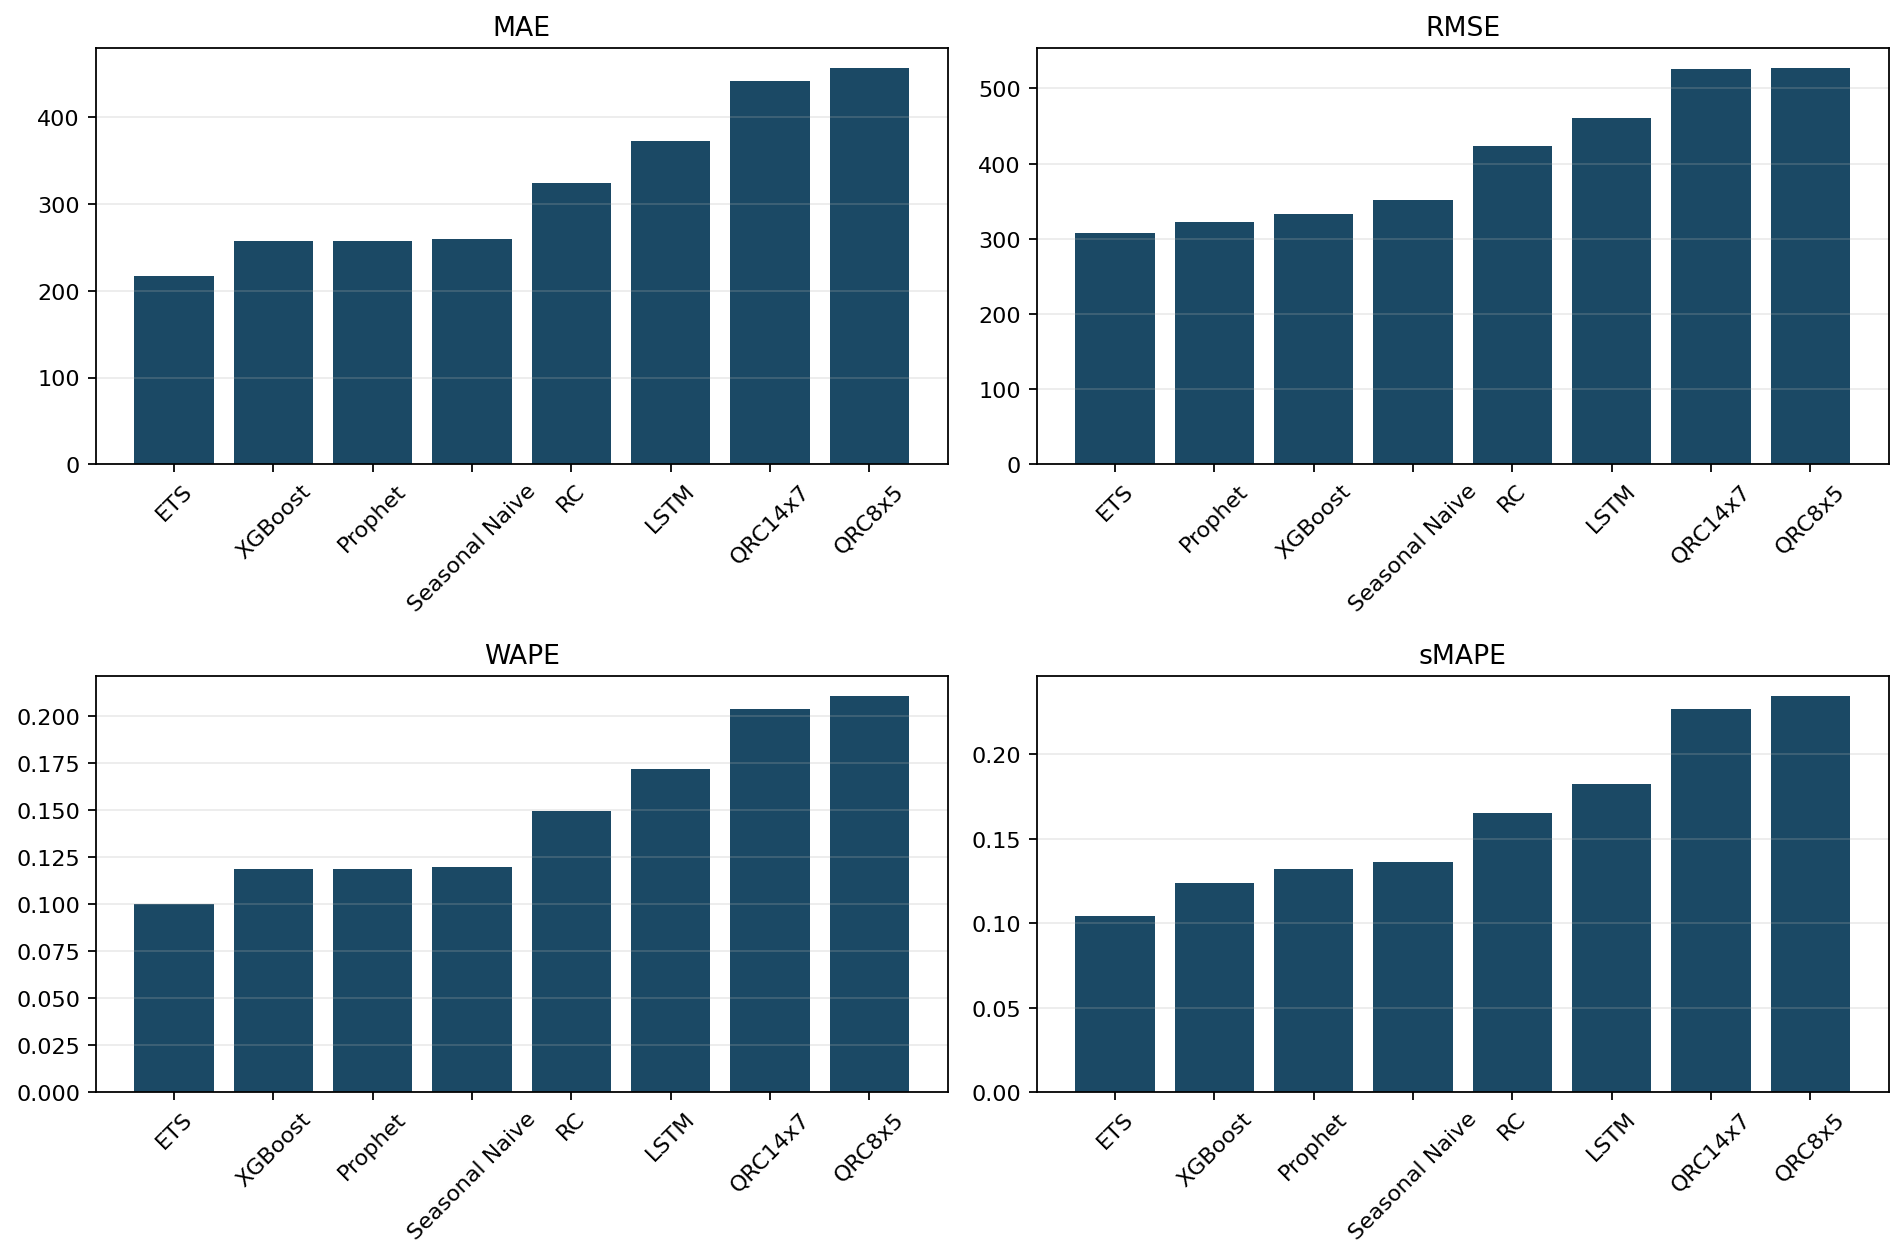
\includegraphics[keepaspectratio,alt={Comparacao visual das metricas do benchmark completo.}]{computational_results_20260402_222902/benchmark_metric_bars.png}}

\pandocbounded{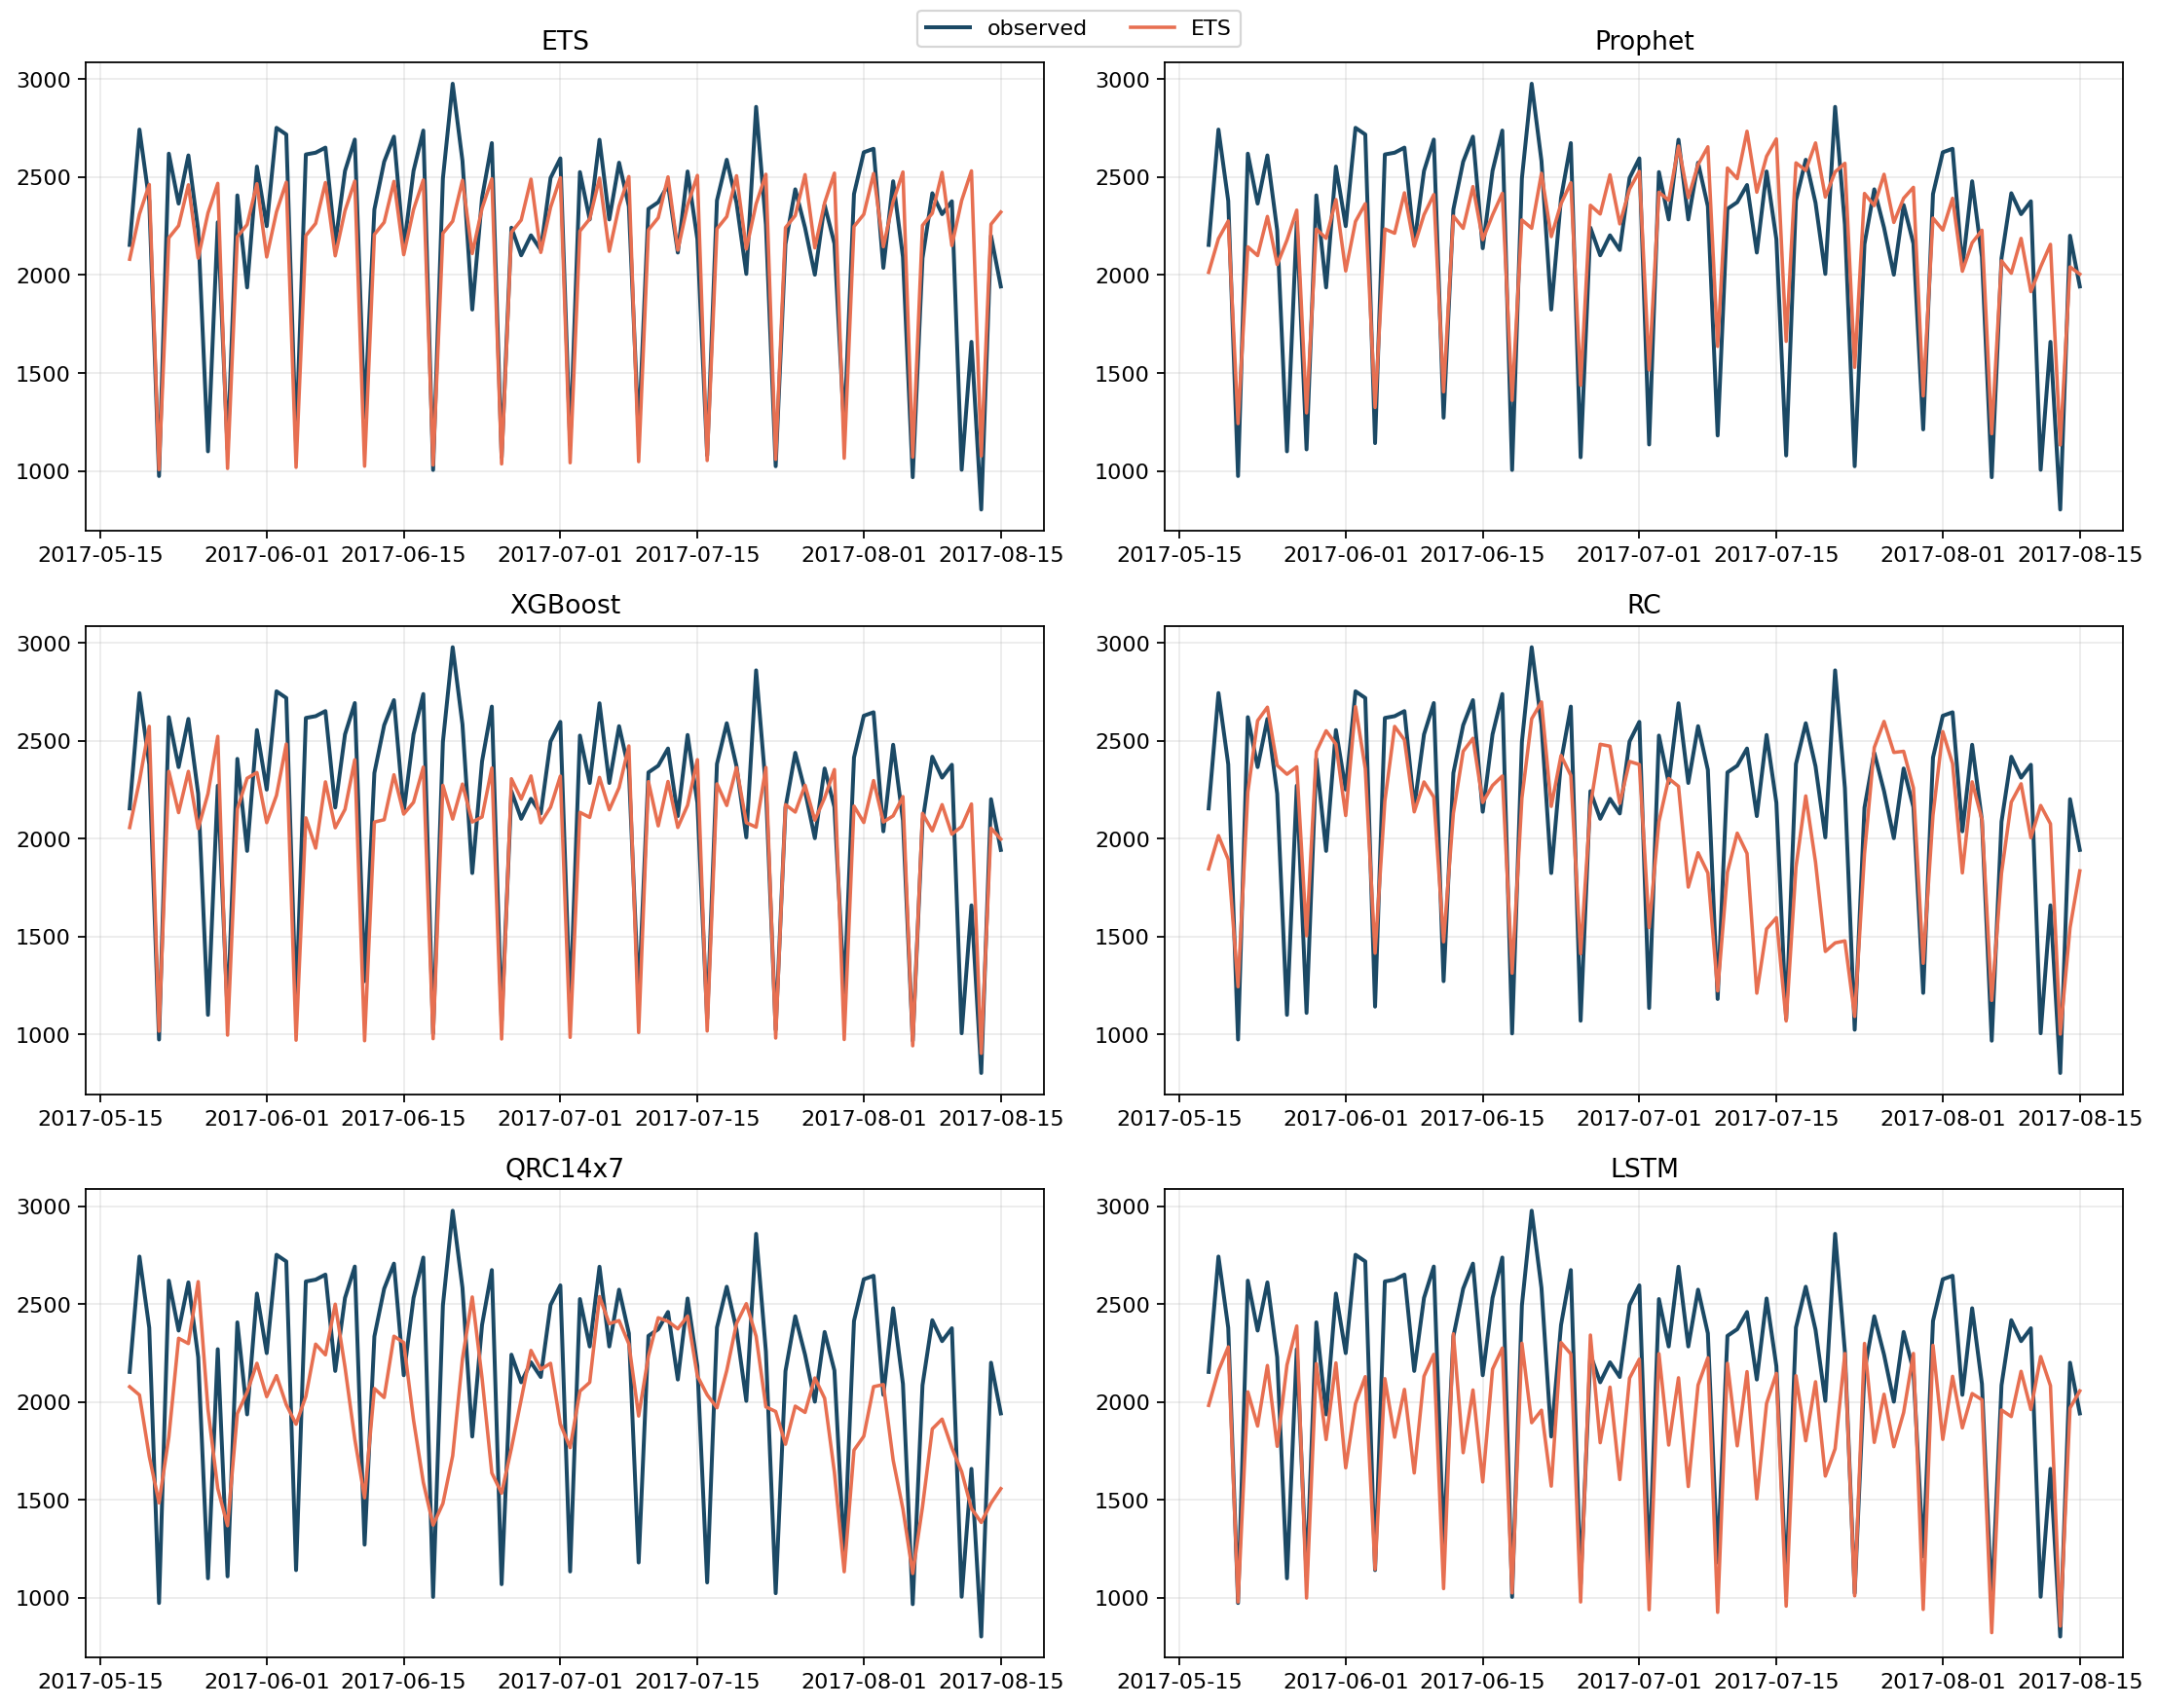
\includegraphics[keepaspectratio,alt={Grade de previsoes dos diferentes modelos no mesmo bloco de teste.}]{computational_results_20260402_222902/benchmark_forecast_grid.png}}

\subsection{6. Leitura dos resultados}\label{6-leitura-dos-resultados}

\subsubsection{6.1 ETS na lideranca}\label{61-ets-na-lideranca}

O \texttt{ETS} foi o melhor modelo no recorte em todas as metricas principais. Isso e importante porque mostra que um baseline estatistico bem implementado continua sendo uma referencia dificil de bater.

\subsubsection{6.2 XGBoost e Prophet como faixa intermediaria forte}\label{62-xgboost-e-prophet-como-faixa-intermediaria-forte}

\texttt{XGBoost} e \texttt{Prophet} formam uma segunda faixa de desempenho. Ambos ficaram muito proximos do \texttt{Seasonal\ Naive} em algumas metricas, mas entregaram um pacote mais robusto no conjunto do benchmark.

\subsubsection{6.3 O que o RC entrega}\label{63-o-que-o-rc-entrega}

O \texttt{RC} superou a \texttt{LSTM}, o que e pedagogicamente interessante. Em um setup pequeno e pouco ajustado, uma rede recorrente treinada por gradiente nao vence automaticamente um reservatorio fixo.

\subsubsection{6.4 O que o QRC entrega}\label{64-o-que-o-qrc-entrega}

O \texttt{QRC} funcionou de ponta a ponta e foi comparado no mesmo recorte de dados. No entanto, ficou abaixo das tecnicas classicas neste benchmark. Isso nao invalida o estudo; ao contrario, torna a comparacao mais honesta.

\subsection{7. O que significa uma comparacao justa}\label{7-o-que-significa-uma-comparacao-justa}

Este benchmark so e didaticamente util porque respeita tres regras:

\begin{enumerate}
\def\labelenumi{\arabic{enumi}.}
\tightlist
\item
  todos os modelos usam os mesmos dados;
\item
  todos produzem previsao para os mesmos \texttt{90} dias;
\item
  todos sao julgados pelas mesmas metricas.
\end{enumerate}

Isso evita a narrativa enganosa de que um modelo "venceu" porque recebeu mais contexto ou uma tarefa mais facil.

\subsection{8. Passo-a-passo para reproduzir o benchmark}\label{8-passo-a-passo-para-reproduzir-o-benchmark}

A reproducao pode ser feita em lotes, executando um script por familia:

\begin{verbatim}
python code/baselines/seasonal_naives/run.py
python code/baselines/ets/run.py
python code/baselines/prophet/run.py
python code/classical/xgboost/run.py
python code/classical/lstm/run.py
python code/rc/run.py
python code/qrc/run.py
\end{verbatim}

Os testes associados seguem a mesma organizacao:

\begin{verbatim}
pytest code/baselines/seasonal_naives/test_model.py
pytest code/baselines/ets/test_model.py
pytest code/baselines/prophet/test_model.py
pytest code/classical/xgboost/test_model.py
pytest code/classical/lstm/test_model.py
pytest code/rc/test_model.py
pytest code/qrc/test_model.py
pytest code/qrc/test_objective.py
\end{verbatim}

\subsection{9. Checklist de boas praticas}\label{9-checklist-de-boas-praticas}

O artigo deixa um checklist minimo para os proximos experimentos:

\begin{itemize}
\tightlist
\item
  manter o split temporal fixo;
\item
  registrar metricas em arquivo;
\item
  salvar previsoes e figuras;
\item
  documentar hiperparametros;
\item
  nao comparar RC e QRC apenas com baselines fracos.
\end{itemize}

\subsection{10. Regras herdadas para a fase QRC}\label{10-regras-herdadas-para-a-fase-qrc}

Quando chegarmos ao QRC, duas regras deste benchmark continuam valendo:

\begin{enumerate}
\def\labelenumi{\arabic{enumi}.}
\tightlist
\item
  o QRC deve ser comparado com as tecnicas classicas ja implementadas;
\item
  o mesmo recorte de dados deve ser mantido, mesmo que o reservatorio quantico simplifique sua representacao interna.
\end{enumerate}

Isso e o que transforma o estudo final em um artigo de ensino serio, e nao em uma demonstracao isolada.

\subsection{11. Conclusao}\label{11-conclusao}

O benchmark consolidado da serie esta agora estabelecido. Ele mostra que a competicao relevante para RC e QRC nao e contra referencias artificiais, mas contra modelos classicos fortes e bem executados. Isso torna a rota ate QRC intelectualmente mais exigente, mas tambem muito mais valiosa.

\subsection{Entregaveis associados no repositorio}\label{entregaveis-associados-no-repositorio}

\begin{itemize}
\tightlist
\item
  benchmark consolidado: \texttt{code/RESULTS.md}
\item
  implementacoes: \texttt{code/baselines/}, \texttt{code/classical/}, \texttt{code/rc/}, \texttt{code/qrc/}
\item
  artefatos comparativos deste artigo: \texttt{computational\_results\_20260402\_222902/}
\end{itemize}

\subsection{Referencias}\label{referencias}

\begin{itemize}
\tightlist
\item
  Hyndman, R. J.; Athanasopoulos, G. Forecasting: Principles and Practice.
\item
  Taylor, S. J.; Letham, B. Forecasting at Scale.
\item
  Chen, T.; Guestrin, C. XGBoost: A scalable tree boosting system.
\item
  Hochreiter, S.; Schmidhuber, J. Long short-term memory.
\item
  Jaeger, H. The "echo state" approach to analysing and training recurrent neural networks.
\end{itemize}

        \end{document}
